We performed classification experiments on LSA16, RWTH and CIARP  handshape datasets. For each experiment, we split the dataset in training and test sets, with the latter taking 25\% of the samples.  The split was stratified,  maintaining the proportion of samples of each class in both sets.

We applied normalization feature-wise substracting the mean and dividing by the standard deviation of each feature. For data augmentation we used horizontal flipping, a 10 and 30 degree rotation and a resampling of the images creating new versions of them with a different size reducing each image by 10\% and 20\% in width and height. We found that a 10 degree rotation gave better results because a rotation of 30 degrees showed to be too high for the nature of the datasets.

We made multiple experiments with Prototypical Networks and DenseNet to find out which hyperparameter configuration was the best for each dataset: with and without data augmentation. We describe the hyper parameters for each model/dataset combination.

\subsection{Prototypical Network}

As mentioned in section \ref{models:protonet}, we can use Prototypical Networks' ability to work with small datasets even if all samples are labeled.

Therefor we experimented with Prototypical Networks using an embedding architecture composed of four convolutional blocks. Each block comprises a \{64, 128\}-filter $3 x 3$ convolution, batch normalization layer, a ReLU nonlinearity and a $2 x 2$ max-pooling layer.

We used the same encoder for embedding both support and query points. All of our models were trained  with the ADAM\cite{Adam} optimizer. We used an initial learning rate of $10^{-3}$ and cut the learning rate in half every 2000 episodes.

We trained prototypical networks using Euclidean distance in the 1-shot and 5-shot scenarios with training episodes containing 16, 20 and 10 classes (for LSA16, RWTH and CIARP respectively) and 5 query points per class. We found it advantageous to match the same value of n for train and test scenarios, and to use a higher value of k (more classes) per training episode. We computed classification accuracy for our models by averaging over 1000 randomly generated episodes from the test set.

In the experiments performed with RWTH we used the same four-block embedding architecture by adding an eight-block architecture with the same layer composition with the idea of analyzing the need to increase the size of the network given the difficulty of the dataset. The difference in the results obtained in 1-shot and 5-shot scenarios for this dataset was very large. We found that 5-shot scenarios gave better results. Using this discovery we only used 5-shot learning in the remaining experiments.

The best configurations for all datasets is the 5-shot scenario with equals n for train and test scenarios by using more than or equal to 5 classes per training episode. Better results were obtained when the number of classes approaches the total amount of classes in the dataset except on CIARP where the best results were obtained when the number of classes per training episode is 5. In addition, the best configurations of the embedding architecture is a 64-filter for all datasets.

\subsection{Wide-DenseNet}

We employed a variation on DenseNet called Wide-DenseNet which follows the strategy used by wide residual networks.\cite{He2015DeepRL}.

We employed a Wide-DenseNet including SE blocks after each dense and transition block. We performed a grid search of hyperparameters to find the model with the best accuracy, averaged over all datasets. We tried growth rate values of 32, 64 and 128 and depth of dense layers of no more than [6,12,24,16], where each number represents the number of dense blocks.

We trained the models using a batch size of 16, an initial learning rate of $10^{-3}$ with categorical cross entropy optimizer and 400 epochs with a maximum patience of 25. The resulting model used a growth rate of 64 and two dense blocks with 6 and 12 layers respectively,  for all datasets.

\subsection{Results}

In table \ref{tab:results}, we can observe that all models have a lower accuracy on the RWTH dataset, which is expected since it has more classes, unsegmented hand images and class imbalances. Prototypical Networks have similar accuracy for LSA16 and CIARP datasets beating the rest of the models, also expected since both datasets have very few examples. For LSA16 they achieve better accuracy than VGG16 and DenseNet; and for CIARP they achieve similar or better accuracy than LeNet CNN and DenseNet. The accuracy of DenseNet on the RWTH is slightly bigger than for other models. Our hypothesis was that Prototypical Networks obtained low accuracy because the images of the hands were unsegmented. It should be noted that the use of data augmentation did not bring significant improvements in the accuracy obtained in LSA16 and CIARP.

Another fact to consider is that better results were obtained with those parameters that reduced the size of the architectures.

\begin{table}[h!]
\centering
\begin{tabular}{ p{17em} p{6em} p{6em} p{6em}}
\toprule
\emph{Method} & \emph{LSA16} &  \emph{RWTH}  &  \emph{CIARP} \\ \midrule
LeNet \cite{ciarp2018} & - & - & 99.20  \\
Inception (fine-tuning) \cite{koller16} & - & 85.50 \\
VGG16 \cite{quiroga2017study} & 95.92 & 82.88 \\
Inception+SVM (pre-trained) \cite{quiroga2017study} &  93.67 & 78.12 & - \\
DenseNet  & 98.07 & 91.10 & 99.93 \\
DenseNet ++  & 98.90 & \textbf{94.00} & 99.99 \\
Prototypical Networks  & 99.15 & 79.93 & 99.98 \\
Prototypical Networks ++ & \textbf{99.26} & 80.85 & \textbf{100.00} \\
\bottomrule
\end{tabular}
\caption{Accuracy of various convolutional neural network based models on three datasets: LSA16, RWTH and CIARP. Models with "++" used data augmentation as described in this section. \label{tab:results}}
\end{table}

In figure \ref{fig:results_varying_samples}, we can observe the accuracy of Prototypical Networks and DenseNet models trained by varying sample sizes. We performed experiments using the same embedding architectures and configurations described in this section varying the training sample sizes with percentages of 44\%, 67\% and 85\% and a fixed test size of 25\%. From the obtained results, we can see that the performance of the DenseNet models increases as more training examples are provided. From figure \ref{fig:results_varying_samples_rwth} we can see that the DenseNet model trained using data augmentation obtains better results than the one trained without. On the other hand, Prototypical Networks models do not show a significant increase in performance as the percentage of samples increases. In figures \ref{fig:results_varying_samples_rwth} and \ref{fig:results_varying_samples_ciarp} we can observe how the use of data augmentation, on RWTH and CIARP datasets respectively, results in Prototypical Networks models with great accuracy improvement compared to the results obtained on LSA16, figure \ref{fig:results_varying_samples_lsa16}), where the increase of performance from the use of data augmentation is minimal.

\begin{figure}[h]
\begin{tabular}{ccc}
    \subfigure[LSA16]{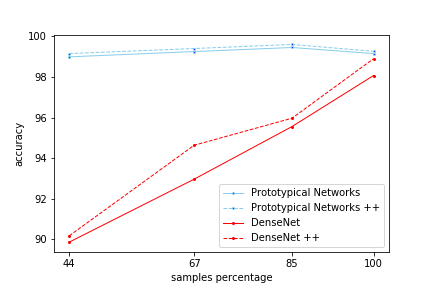
\includegraphics[width=0.32\columnwidth]{results/lsa16.png} \label{fig:results_varying_samples_lsa16}} & \subfigure[RWTH]{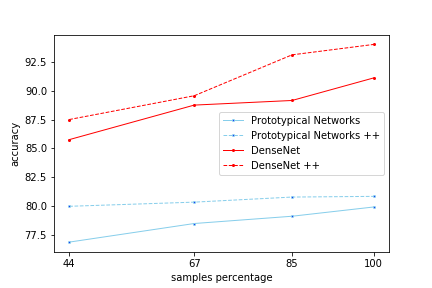
\includegraphics[width=0.32\columnwidth]{results/rwth.png} \label{fig:results_varying_samples_rwth}} & \subfigure[CIARP]{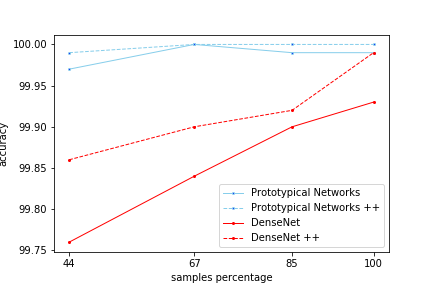
\includegraphics[width=0.32\columnwidth]{results/ciarp.png} \label{fig:results_varying_samples_ciarp}} \\
\end{tabular}
\caption{Accuracy of Prototypical Networks and DenseNet models trained by varying sample sizes on three datasets: LSA16, RWTH and CIARP. Each plot represents a different dataset where the x-axis is the percentage of samples used and the y-axis is the accuracy obtained. Models with "++" used data augmentation as described in this section. \label{fig:results_varying_samples}}
\end{figure}